\documentclass[11pt,a4paper]{article}
\usepackage[margin=26mm]{geometry}
\usepackage[T1]{fontenc}
\usepackage{mathtools,amsthm,bm}
\usepackage{newtxtext,newtxmath}
\usepackage{microtype}
\usepackage{booktabs,enumitem,graphicx,xcolor}
\usepackage{authblk}
\usepackage[hidelinks]{hyperref}
\usepackage[nameinlink,capitalise,noabbrev]{cleveref}
\usepackage{fancyhdr}
\usepackage{caption}

\definecolor{ink}{HTML}{17243A}
\definecolor{muted}{HTML}{526079}
\hypersetup{
  pdftitle={Many-Body Filling Turns Soft Spectral Leakage into a Maintenance Floor},
  pdfauthor={Lluis Eriksson},
  pdfsubject={Exact filled-SSH sum rules, Davies leakage floors, and interaction-stable obstructions}
}
\setlength{\parindent}{1.15em}
\setlength{\parskip}{0.15em}
\emergencystretch=1.5em
\hfuzz=0.5pt
\hbadness=2000
\setlist{nosep,leftmargin=1.8em}
\captionsetup{font=small,labelfont=bf}
\pagestyle{fancy}
\fancyhf{}
\fancyhead[L]{\small\itshape Many-body filling and maintenance floors}
\fancyhead[R]{\small\thepage}
\renewcommand{\headrulewidth}{0.3pt}

\newtheorem{theorem}{Theorem}[section]
\newtheorem{lemma}[theorem]{Lemma}
\newtheorem{proposition}[theorem]{Proposition}
\newtheorem{corollary}[theorem]{Corollary}
\theoremstyle{remark}
\newtheorem{remark}[theorem]{Remark}
\newcommand{\D}{\mathcal D}
\newcommand{\id}{\mathrm{id}}
\newcommand{\hc}{\mathrm{h.c.}}
\newcommand{\cH}{\mathcal H}
\newcommand{\cL}{\mathcal L}
\newcommand{\cC}{\mathcal C}
\DeclareMathOperator{\supp}{supp}
\DeclareMathOperator{\Tr}{Tr}

\title{\textcolor{ink}{\bfseries Many-Body Filling Turns Soft Spectral Leakage\\into a Maintenance Floor}\\[0.5em]
\large Exact Filled-SSH Sum Rules and an Interaction-Stable Obstruction}
\author{Lluis Eriksson}
\affil{Independent Researcher}
\date{13 July 2026}

\begin{document}
\maketitle

\begin{abstract}
Soft spectral filtering has a more severe effect at finite filling than in a dilute edge-mode code.  We consider two odd Su--Schrieffer--Heeger (SSH) rails, fill every negative-energy orbital, and encode one additional fermion in the zero mode of either rail.  The code has fixed total number and supports physical coherence.  For a boundary transfer at a site with zero-mode weight $w_x$, the desired logical Davies line has squared matrix element $w_x^2$.  We prove the exact many-body leakage identity
\[
 W_{\mathrm{leak}}^{\mathrm{filled}}(x)
 =\frac{1+2w_x-3w_x^2}{4}.
\]
At the remote boundary, $w_x=\Theta(\zeta^{2\ell})$, so the logical line is $\Theta(\zeta^{4\ell})$ while the summed particle--hole leakage tends to $1/4$.  This differs qualitatively from the dilute identity $w_x(1-w_x)=\Theta(\zeta^{2\ell})$.

For a Davies filter whose off-target tail is $\epsilon_\ell=\exp[-q\ell+o(\ell)]$, the bounded-latency exact-refresh power therefore obeys the exponent law
\[
 \lim_{\ell\to\infty}-\frac1\ell\log P_{\ell,\tau}
 =\min\{4m,q\},\qquad m=-\log\zeta,
\]
under explicit uniform envelope and resource-ledger assumptions.  A width-independent tail (a special case with $q=0$) produces a nonzero maintenance floor, rather than merely halving the membrane exponent.  More generally, $q=0$ means only that the decay is subexponential.  Every nonzero tail also makes the exact rapid-refresh limit logarithmically singular at each fixed width.

The floor is not a free-fermion accident.  For arbitrary interacting number-conserving rails, we prove an exact static identity expressing leakage as a local occupation product minus the logical matrix element.  Uniform finite filling and remote edge indistinguishability force a positive leakage floor.  A new local spectral-window lemma then places a fixed fraction of that weight in a width-independent Bohr-frequency window using only a commutator norm.  Consequently, any bath tail bounded below on that window yields an interaction-stable Davies leakage floor.  Quasi-local spectral flow shows persistence in a neighborhood of a symmetry-preserving gapped SSH phase.  Exact diagonalization of the interacting spinless SSH chain shows that repulsive and attractive interactions change the observed edge localization exponent while the leakage is already driven close to $1/4$ at accessible widths.
\end{abstract}

\section{Result and novelty boundary}

The distinction between a dilute code and a filled many-body code is easy to miss.  In a one-particle sector, annihilating at the remote boundary first has to find the localized edge particle.  This supplies one exponentially small factor before any final state is selected.  At half filling, the same local operator can remove a sea particle and create a particle--hole excitation with order-one total weight.  Selecting the desired zero mode on both rails remains exponentially unlikely, but leaking into the orthogonal many-body spectrum does not.

The paper establishes the following chain:
\[
\begin{gathered}
\text{chiral projector identity}
\Longrightarrow
\text{exact filled-SSH leakage sum rule}
\Longrightarrow
W_{\mathrm{leak}}\to\tfrac14,\\
\text{soft Davies tail}
\Longrightarrow
\min\{4m,q\}
\Longrightarrow
\text{width-independent tail}\Longrightarrow\text{maintenance floor},\\
\text{finite filling + remote edge indistinguishability}
\Longrightarrow\text{interacting static floor},\\
\text{interacting static floor + locality}
\Longrightarrow\text{spectral-window Davies floor}.
\end{gathered}
\]

The nonanalyticity of entropy at rank-deficient states is standard and is treated systematically by Grace and Guha~\cite{GraceGuha}.  Davies generators, detailed balance, and Spohn entropy production are also classical~\cite{Davies,Spohn}.  Half-filled SSH ladders and the operational entanglement of filled edge states have been studied by Monkman and Sirker~\cite{MonkmanSirker}; we do not claim that finite filling or its edge physics is new.  A companion paper converts first-order support leakage into a rapid-maintenance singularity and derives the dilute SSH law $\min\{4m,2m+q\}$~\cite{ErikssonLeakage}.  Existing autonomous-QEC bounds concern logical error versus engineered correction rate~\cite{ShtankoEtAl}; they do not contain the filled-background line--continuum identity proved here.  The new results are specifically the exact leakage sum rule, its Davies filter consequence, the exponent collapse to $\min\{4m,q\}$, and the local spectral-window obstruction.  We do not claim a microscopic weak-coupling limit uniform in $\ell$, autonomous work-only optimality, or a general proof that an arbitrary interacting SPT phase has a nonzero remote logical prefactor.

\section{Odd SSH rails at half filling}

\subsection{Single-particle geometry}

An odd SSH rail~\cite{SSH} has sites $A_0,\ldots,A_\ell$ and $B_0,\ldots,B_{\ell-1}$.  Subtracting an irrelevant rail offset, its one-body Hamiltonian is
\[
 h_\ell=\sum_{j=0}^{\ell-1}
 \bigl(t_1|A_j\rangle\langle B_j|+t_2|A_{j+1}\rangle\langle B_j|+\hc\bigr),
 \qquad 0<t_1<t_2.
\]
Put $\zeta=t_1/t_2<1$ and $m=-\log\zeta$.  Chiral symmetry is implemented by
\[
 \Gamma|A_j\rangle=|A_j\rangle,\qquad
 \Gamma|B_j\rangle=-|B_j\rangle,\qquad
 \Gamma h_\ell\Gamma=-h_\ell.
\]
There is a unique zero mode
\[
 |\psi\rangle=\mathcal N_\ell\sum_{j=0}^{\ell}(-\zeta)^j|A_j\rangle,
 \qquad
 \mathcal N_\ell^2=\frac{1-\zeta^2}{1-\zeta^{2\ell+2}}.
\]
For a site $x$, write $w_x=|\langle x|\psi\rangle|^2$.  Let $\Pi_0=|\psi\rangle\langle\psi|$ and let $\Pi_\pm$ be the positive- and negative-energy spectral projectors of $h_\ell$.

\begin{lemma}[Chiral diagonal splitting]\label{lem:chiral}
For every $A$-sublattice site $x$,
\[
 \langle x|\Pi_-|x\rangle
 =\langle x|\Pi_+|x\rangle
 =\frac{1-w_x}{2}.
\]
\end{lemma}

\begin{proof}
Chiral symmetry maps the positive spectral subspace unitarily onto the negative spectral subspace, hence $\Gamma\Pi_+\Gamma=\Pi_-$.  Since $\Gamma|x\rangle=|x\rangle$ on the $A$ sublattice, the two diagonal matrix elements coincide.  Completeness gives $\Pi_-+\Pi_++\Pi_0=1$, so their sum is $1-w_x$.
\end{proof}

At the far boundary $x=A_\ell$,
\begin{equation}\label{eq:wfar}
 w_{\ell,\mathrm{far}}
 =\frac{(1-\zeta^2)\zeta^{2\ell}}{1-\zeta^{2\ell+2}},
 \qquad
 (1-\zeta^2)\zeta^{2\ell}\le w_{\ell,\mathrm{far}}\le\zeta^{2\ell}.
\end{equation}

\subsection{Filled rails and the fixed-number code}

Let $|g_\ell\rangle$ be the Slater determinant filling all $\ell$ negative-energy orbitals, and let
\[
 |e_\ell\rangle=f_0^\dagger|g_\ell\rangle
\]
also occupy the zero mode.  These states contain $\ell$ and $\ell+1$ particles.  By \cref{lem:chiral}, for $x$ on the $A$ sublattice,
\begin{equation}\label{eq:occupations}
 \langle g_\ell|n_x|g_\ell\rangle=\frac{1-w_x}{2},
 \qquad
 \langle e_\ell|n_x|e_\ell\rangle=\frac{1+w_x}{2},
 \qquad
 \langle g_\ell|a_x|e_\ell\rangle=\psi_x.
\end{equation}

Take two identical rails, with optional number offsets $\Delta_0N_0$ and $\Delta_1N_1$.  The logical code is
\[
 |0_L\rangle=|e_\ell\rangle_0\otimes|g_\ell\rangle_1,
 \qquad
 |1_L\rangle=|g_\ell\rangle_0\otimes|e_\ell\rangle_1.
\]
Both states have total number $2\ell+1$ and the same fermion parity.  Their coherence is therefore physical.  At corresponding boundary sites define the even, number-conserving transfer
\[
 S_x=a_{1,x}^\dagger a_{0,x}.
\]
The desired logical Bohr frequency is $\delta=\Delta_1-\Delta_0$.

\section{Exact many-body leakage sum rule}

Let $P_L=|0_L\rangle\langle0_L|+|1_L\rangle\langle1_L|$ and $Q_L=1-P_L$.

\begin{theorem}[Filled-SSH transfer identity]\label{thm:filledidentity}
For a transfer from rail zero to rail one at an $A$-sublattice site $x$,
\begin{align}
 W_{\log}(x)
 &:=|\langle1_L|S_x|0_L\rangle|^2=w_x^2,\label{eq:wlog}\\
 W_{\mathrm{tot}}(x)
 &:=\|S_x|0_L\rangle\|^2=\frac{(1+w_x)^2}{4},\label{eq:wtot}\\
 W_{\mathrm{leak}}(x)
 &:=\|Q_LS_x|0_L\rangle\|^2
 =\frac{1+2w_x-3w_x^2}{4}.\label{eq:wleak}
\end{align}
The reverse transfer obeys the same identities.
\end{theorem}

\begin{proof}
Factorization across rails and \cref{eq:occupations} give
\[
 \langle1_L|S_x|0_L\rangle
 =\langle g_\ell|a_x|e_\ell\rangle
  \langle e_\ell|a_x^\dagger|g_\ell\rangle
 =|\psi_x|^2=w_x.
\]
The graded tensor-product signs are uniform and disappear after taking the modulus.  Next,
\[
 S_x^\dagger S_x=n_{0,x}(1-n_{1,x})
\]
on the two-rail Fock space.  Hence
\[
 \|S_x|0_L\rangle\|^2
 =\frac{1+w_x}{2}\left(1-\frac{1-w_x}{2}\right)
 =\frac{(1+w_x)^2}{4}.
\]
Orthogonally decomposing $S_x|0_L\rangle$ into its logical and nonlogical components yields \cref{eq:wleak}.
\end{proof}

The leakage can also be resolved into three mutually orthogonal processes:
\begin{center}
\begin{tabular}{@{}lc@{}}
\toprule
process & summed squared weight\\
\midrule
zero mode $\to$ positive band & $w_x(1-w_x)/2$\\
negative band $\to$ zero mode & $w_x(1-w_x)/2$\\
negative band $\to$ positive band & $(1-w_x)^2/4$\\
\bottomrule
\end{tabular}
\end{center}
The last line is the finite-density channel absent in the dilute code.

\begin{corollary}[Remote leakage floor]\label{cor:floor}
At $x=A_\ell$,
\[
 W_{\log}=\Theta(\zeta^{4\ell}),
 \qquad
 W_{\mathrm{leak}}=\frac14+O(\zeta^{2\ell}).
\]
In particular, $W_{\mathrm{leak}}\ge1/4$ for all sufficiently large $\ell$.
\end{corollary}

\begin{remark}[Dilute versus filled]
For the one-particle dual-rail code, completeness gives $W_{\mathrm{leak}}^{\mathrm{dilute}}=w_x(1-w_x)$.  Filling the negative band adds the particle--hole term $(1-w_x)^2/4$ and changes a remote exponential tail into a constant.  This is a change of asymptotic class, not a prefactor correction.
\end{remark}

\section{Davies rates under a soft filter}

Couple the boundary operator $A_x=S_x+S_x^\dagger$ weakly to a thermal reservoir.  At each fixed $\ell$, the secular Davies generator has jump operators $A_\omega$ and nonnegative spectral weights $G_\ell(\omega)$.  The logical line lies at $\pm\delta$.  All free-fermion particle--hole leakage frequencies lie in a compact set independent of $\ell$ because the SSH bands have width bounded by $t_1+t_2$.

We impose the following explicit filter envelope.  There are constants $g_\pm,c_\pm>0$, independent of $\ell$, and a sequence $0\le\epsilon_\ell\le1$ such that
\begin{align}
 g_-\le G_\ell(\pm\delta)\le g_+,&\label{eq:logicalenvelope}\\
 c_-\epsilon_\ell\le G_\ell(\omega)\le c_+\epsilon_\ell
 &\quad\text{for every active leakage frequency }\omega.\label{eq:tailenvelope}
\end{align}
KMS-related signs may have different constants; this does not affect the conclusions.

\begin{theorem}[Davies line--continuum separation]\label{thm:daviesweights}
Let $a_{\ell,\log}$ and $a_{\ell,\mathrm{leak}}$ denote the total desired logical and outward leakage coefficients generated by the boundary coupling, for a logical target whose two populations are bounded below by a constant.  Then
\[
 a_{\ell,\log}=\Theta(w_{\ell,\mathrm{far}}^2),
 \qquad
 a_{\ell,\mathrm{leak}}=\Theta(\epsilon_\ell).
\]
The constants are uniform in $\ell$.
\end{theorem}

\begin{proof}
The desired Bohr component contains the matrix element in \cref{eq:wlog}; \cref{eq:logicalenvelope} therefore gives two-sided multiples of $w_{\ell,\mathrm{far}}^2$.  The remaining Bohr components are mutually orthogonal after summing over final eigenstates.  Their unweighted total is exactly \cref{eq:wleak}.  Applying \cref{eq:tailenvelope} term by term and using \cref{cor:floor} gives two-sided multiples of $\epsilon_\ell$.  The two transfer directions cover both logical populations.  Coherences do not cancel the positive sum because the opposite rail-number changes land in orthogonal leakage sectors.
\end{proof}

\begin{corollary}[Rate exponent collapse]\label{cor:rateexponent}
If
\[
 \epsilon_\ell=\exp[-q\ell+o(\ell)],\qquad q\in[0,\infty],
\]
then the total boundary dissipation coefficient has exponential rate
\[
 \lim_{\ell\to\infty}-\frac1\ell
 \log(a_{\ell,\log}+a_{\ell,\mathrm{leak}})
 =\min\{4m,q\}.
\]
An exact filter is represented by $q=\infty$.
\end{corollary}

\section{Maintenance consequences}

\subsection{Rapid exact refresh}

Let $T_t^{(\ell)}=\exp(t\cL_\ell)$ and let $\rho_\ell$ be faithful on the two-dimensional logical code and zero on its orthogonal complement.  Set $P=P_L$, $Q=1-P$, and
\[
 a_\ell=\Tr[Q\cL_\ell(\rho_\ell)].
\]

\begin{lemma}[Boundary free-energy loss]\label{lem:boundaryF}
For a finite-dimensional Hamiltonian and $a_\ell>0$,
\[
 F(\rho_\ell)-F(T_t^{(\ell)}\rho_\ell)
 =k_{\mathrm B}T\,a_\ell t\log(1/t)+O_\ell(t)
 \qquad(t\downarrow0).
\]
\end{lemma}

\begin{proof}
Positivity gives $Q\cL_\ell(\rho_\ell)Q\ge0$ with trace $a_\ell$.  The new kernel eigenvalues are $t$ times the positive eigenvalues of this block, up to $O(t^2)$.  Their entropy contribution is $-a_\ell t\log t+O_\ell(t)$.  Eigenvalues inside the original support and the energy expectation vary analytically at order $t$.  Combining the terms gives the formula.  This is the support-extending branch of standard entropy perturbation theory~\cite{GraceGuha}.
\end{proof}

Under the explicit fresh-target-cell ledger, the optimal exact replacement cost is the free-energy loss.  Thus any $\epsilon_\ell>0$ gives $a_\ell>0$ by \cref{thm:daviesweights} and the rapid power diverges logarithmically at every fixed width.  This is not a statement about work-only autonomous control.

\subsection{Fixed latency}

Fix a refresh period $0<\tau\le\tau_0$.  Let
\[
 P_{\ell,\tau}
 =\frac{F(\rho_\ell)-F(T_\tau^{(\ell)}\rho_\ell)}{\tau}.
\]
We now make the uniformity assumptions precise.  The code projector $P=P_{L,\ell}$ is assumed to be a sum of complete spectral projections of $H_\ell$, separated from $Q=1-P$ by an isolated band.  Thus the Davies dynamics preserves the $P\oplus Q$ block decomposition even in the presence of degeneracies.  We work in the interaction picture, where the Hamiltonian commutator drops out of both $q_\ell(t)=\Tr[Q\rho_\ell(t)]$ and the dissipative trace-norm estimates.  The exactly filtered restriction is
\[
 P\widetilde{\cL}_\ell^{(0)}(PXP)P
 =w_{\ell,\mathrm{far}}^2\cL_{\log,0}(X),
\]
and the faithful logical target has a normalized entropy-production coefficient bounded below independently of $\ell$.

For the Davies jumps $J_{\ell,\omega}=G_\ell(\omega)^{1/2}A_{\ell,\omega}$ define the positive crossing maps
\begin{align}
 \Phi_\ell^{\mathrm{out}}(X)
 &=\sum_\omega QJ_{\ell,\omega}PXPJ_{\ell,\omega}^\dagger Q,\\
 \Phi_\ell^{\mathrm{in}}(Y)
 &=\sum_\omega PJ_{\ell,\omega}QYQJ_{\ell,\omega}^\dagger P.
\end{align}

\begin{lemma}[Uniform crossing norms]\label{lem:crossingnorm}
Under \cref{eq:tailenvelope},
\[
 \|\Phi_\ell^{\mathrm{out}}\|_{1\to1}
 +\|\Phi_\ell^{\mathrm{in}}\|_{1\to1}
 \le C_\times\epsilon_\ell.
\]
The interaction-picture Davies dissipator also obeys
\[
 \|\widetilde{\cL}_\ell\|_{1\to1}\le M_*
\]
with constants independent of $\ell$ and of Bohr-frequency degeneracies.
\end{lemma}

\begin{proof}
For a positive map $\Phi(X)=\sum_jB_jXB_j^\dagger$, its induced trace norm is
\[
 \|\Phi\|_{1\to1}=\|\Phi^*(1)\|_\infty
 =\left\|\sum_jB_j^\dagger B_j\right\|_\infty.
\]
Every $P\leftrightarrow Q$ component lies in the leakage envelope, hence
\[
 \sum_\omega PJ_{\ell,\omega}^\dagger QJ_{\ell,\omega}P
 \le c_+\epsilon_\ell
 \sum_\omega PA_{\ell,\omega}^\dagger A_{\ell,\omega}P.
\]
The sum on the right is a sub-sum of the energy pinching of $A_x^\dagger A_x$ and is bounded by $\|A_x\|^2P$.  This proves the outward estimate; the incoming estimate is identical, using the KMS-related upper envelope.  The same pinching identity, now without $P,Q$, bounds the completely positive and anticommutator pieces of the full dissipator by a constant multiple of $\sup_\omega G_\ell(\omega)\|A_x\|^2$.  Combining degenerate transitions inside a single $A_{\ell,\omega}$ changes neither estimate, so no number-of-modes factor appears.
\end{proof}

\begin{lemma}[Uniform fixed-time leakage]\label{lem:fixedleakage}
There exist $\tau_0,c,C>0$, independent of $\ell$, such that
\[
 c\tau\epsilon_\ell
 \le q_\ell(\tau):=\Tr[Q T_\tau^{(\ell)}(\rho_\ell)]
 \le C\tau\epsilon_\ell
\]
for $0<\tau\le\tau_0$ and all sufficiently large $\ell$.
\end{lemma}

\begin{proof}
Block preservation gives the exact balance equation
\[
 q_\ell'(t)
 =\Tr\Phi_\ell^{\mathrm{out}}(P\rho_\ell(t)P)
 -\Tr\Phi_\ell^{\mathrm{in}}(Q\rho_\ell(t)Q).
\]
At $t=0$, \cref{thm:daviesweights} gives
\[
 a_-\epsilon_\ell\le q_\ell'(0)\le a_+\epsilon_\ell.
\]
Contractivity and \cref{lem:crossingnorm} imply
\begin{align*}
 \bigl|\Tr\Phi_\ell^{\mathrm{out}}(P\rho_\ell(t)P)-q_\ell'(0)\bigr|
 &\le C_\times\epsilon_\ell M_*t,\\
 0\le\Tr\Phi_\ell^{\mathrm{in}}(Q\rho_\ell(t)Q)
 &\le C_\times\epsilon_\ell q_\ell(t).
\end{align*}
The upper differential inequality first gives $q_\ell(t)\le C\epsilon_\ell t$ on a width-independent interval by Gronwall.  Substitution into the lower inequality gives
\[
 q_\ell'(t)\ge a_-\epsilon_\ell-C_0\epsilon_\ell t-C_1\epsilon_\ell^2t.
\]
Choose $\tau_0$ so that the last two terms are at most $a_-\epsilon_\ell/2$, then integrate.  The upper bound follows from the corresponding upper inequality.
\end{proof}

\begin{lemma}[Free-energy sandwich]\label{lem:Fsandwich}
Assume in addition that all active boundary-transfer Bohr frequencies lie in a width-independent compact interval and that $\log d_{Q,\ell}\le c_d\ell$.  For $0<\tau\le\tau_0$ and sufficiently small $\epsilon_\ell$,
\[
 c_1\tau w_{\ell,\mathrm{far}}^2
 +k_{\mathrm B}T\bigl[h_2(q_\ell(\tau))-C_1q_\ell(\tau)\bigr]
 \le \tau P_{\ell,\tau}
 \le
 C_2\tau w_{\ell,\mathrm{far}}^2
 +k_{\mathrm B}T\bigl[h_2(q_\ell(\tau))+C_3\ell q_\ell(\tau)\bigr].
\]
Here $h_2$ is binary entropy and all constants are width independent.
\end{lemma}

\begin{proof}
Because $P$ is a sum of complete spectral projections, the secular evolution is block diagonal:
\[
 T_\tau^{(\ell)}(\rho_\ell)
 =(1-q)\sigma_\ell\oplus q\chi_\ell.
\]
Consequently,
\[
 S((1-q)\sigma\oplus q\chi)=h_2(q)+(1-q)S(\sigma)+qS(\chi).
\]
Let $\eta_\ell(\tau)$ be the evolution with the crossing jumps removed.  Duhamel's formula and \cref{lem:crossingnorm} give
\[
 \|P T_\tau^{(\ell)}(\rho_\ell)P-\eta_\ell(\tau)\|_1
 \le C\tau\epsilon_\ell.
\]
The target is faithful on the two-dimensional code, so for sufficiently small $\tau_0$ both normalized logical blocks have eigenvalues bounded below by a width-independent constant.  Entropy and energy are therefore Lipschitz on this block.  Strictly positive normalized logical entropy production gives
\[
 c_1\tau w_{\ell,\mathrm{far}}^2
 \le F(\rho_\ell)-F(\eta_\ell(\tau))
 \le C_2\tau w_{\ell,\mathrm{far}}^2.
\]
For the leakage correction, the compact Bohr window bounds the energy transported per jump.  Equivalently, the Davies energy flux is a frequency-weighted positive sum, so its absolute crossing contribution is at most $Cq_\ell(\tau)$.  The logical-block Duhamel error is of the same order by \cref{lem:fixedleakage}.  In the entropy identity, $qS(\chi)\ge0$ gives the lower bound, while
\[
 qS(\chi)\le q\log d_{Q,\ell}\le c_d\ell q
\]
gives the upper bound.  Collecting the analytic $O(q)$ terms proves the sandwich.
\end{proof}

\begin{theorem}[Many-body exponent collapse]\label{thm:powerexponent}
Suppose $\epsilon_\ell=\exp[-q\ell+o(\ell)]$ and the assumptions above hold.  For every fixed $0<\tau\le\tau_0$,
\[
 \boxed{
 \lim_{\ell\to\infty}-\frac1\ell\log P_{\ell,\tau}
 =\min\{4m,q\}.}
\]
If $q=0$, the displayed exponent is zero.  A positive width-independent lower bound on $P_{\ell,\tau}$ requires the additional condition $\liminf_{\ell\to\infty}\epsilon_\ell>0$ (and a sufficiently weak tail so that the uniform small-time estimates apply).
\end{theorem}

\begin{proof}
By \cref{eq:wfar}, the logical term has rate $4m$.  By \cref{lem:fixedleakage}, $q_\ell(\tau)=\exp[-q\ell+o(\ell)]$.  If $q>0$, then
\[
 h_2(q_\ell(\tau))
 =q_\ell(\tau)\log(1/q_\ell(\tau))+O(q_\ell(\tau))
\]
has rate $q$; polynomial factors in $\ell$ do not alter it.  The sandwich therefore gives the minimum of the two rates, including the equality case $q=4m$.  When $q=0$, the same bounds give exponent zero but allow subexponential decay, for example $\epsilon_\ell=1/\ell$.  If in addition $\liminf_\ell\epsilon_\ell>0$, choose $\tau_0$ and the tail amplitude small enough that the positive binary-entropy term dominates the analytic $O(q_\ell(\tau))$ correction.  Only under this additional condition is the lower bound width independent.
\end{proof}

The two limits again do not commute whenever the tail remains nonzero at each fixed width.  At fixed $\ell$, $\lim_{\tau\downarrow0}P_{\ell,\tau}=\infty$.  At fixed $\tau$, $q>0$ forces the wide-width power to vanish exponentially.  When $q=0$, the exponential rate is zero: the power may vanish subexponentially, and a positive floor follows only if $\liminf_\ell\epsilon_\ell>0$.

\section{An exact interacting leakage identity}

We now discard the free-fermion structure.  On one interacting rail, let $|g_\ell\rangle$ and $|e_\ell\rangle$ be normalized eigenstates in adjacent number sectors.  Define at a boundary site $x$
\[
 \alpha_\ell=\langle g_\ell|a_x|e_\ell\rangle,
 \quad
 n_{e,\ell}=\langle e_\ell|n_x|e_\ell\rangle,
 \quad
 v_{g,\ell}=\langle g_\ell|(1-n_x)|g_\ell\rangle.
\]
Use the same fixed-number two-rail code and transfer $S_x$ as before.

\begin{theorem}[Interacting occupation--leakage identity]\label{thm:interactingidentity}
For arbitrary number-conserving rail Hamiltonians,
\begin{align}
 W_{\log}^{\mathrm{int}}&=|\alpha_\ell|^4,\\
 W_{\mathrm{tot}}^{\mathrm{int}}&=n_{e,\ell}v_{g,\ell},\\
 W_{\mathrm{leak}}^{\mathrm{int}}&=n_{e,\ell}v_{g,\ell}-|\alpha_\ell|^4.
\end{align}
Consequently, if $n_{e,\ell},v_{g,\ell}\ge\nu>0$ and $|\alpha_\ell|\to0$, then
\[
 \liminf_{\ell\to\infty}W_{\mathrm{leak}}^{\mathrm{int}}\ge\nu^2.
\]
\end{theorem}

\begin{proof}
The logical matrix element factorizes into $\alpha_\ell\overline{\alpha_\ell}$.  The identity $S_x^\dagger S_x=n_{0,x}(1-n_{1,x})$ and the product structure of the two rails give the total weight.  Subtracting the squared logical projection gives the leakage identity.  The lower bound is immediate.
\end{proof}

If particle--hole symmetry maps $|g_\ell\rangle$ to $|e_\ell\rangle$, then $v_{g,\ell}=n_{e,\ell}$ and the total weight is $n_{e,\ell}^2$.  The theorem shows precisely which hypothesis replaces free-fermion completeness: finite local filling supplies the floor, while remote edge indistinguishability makes the desired matrix element vanish.

\section{A local spectral-window theorem}

A static leakage floor is useful only if a fixed fraction lies where the bath tail is controlled.  The next result supplies that fraction without counting many-body levels.

\begin{lemma}[Local spectral window]\label{lem:spectralwindow}
Let $H_\ell|0_L\rangle=E_{0,\ell}|0_L\rangle$ and $H_\ell|1_L\rangle=E_{1,\ell}|1_L\rangle$, with $\delta_\ell=E_{1,\ell}-E_{0,\ell}$.  Assume $P_L$ is a spectral projector and put
\[
 v_\ell=Q_LS_x|0_L\rangle,
 \qquad W_\ell=\|v_\ell\|^2.
\]
If
\[
 \|([H_\ell,S_x]-\delta_\ell S_x)|0_L\rangle\|\le K
\]
uniformly in $\ell$, then for every $\Omega>0$,
\[
 \langle v_\ell,
 \mathbf1_{\{|H_\ell-E_{0,\ell}-\delta_\ell|\le\Omega\}}v_\ell\rangle
 \ge W_\ell-\frac{K^2}{\Omega^2}.
\]
In particular, if $W_\ell\ge c_0>0$, choosing $\Omega\ge\sqrt{2}K/\sqrt{c_0}$ places at least $c_0/2$ leakage weight in a width-independent frequency window.
\end{lemma}

\begin{proof}
Because $P_L$ is spectral, $Q_L$ commutes with $H_\ell$.  The centered second moment of the spectral measure of $v_\ell$ is
\begin{align*}
 \|(H_\ell-E_{0,\ell}-\delta_\ell)v_\ell\|^2
 &\le\|(H_\ell-E_{0,\ell}-\delta_\ell)S_x|0_L\rangle\|^2\\
 &=\|([H_\ell,S_x]-\delta_\ell S_x)|0_L\rangle\|^2\le K^2.
\end{align*}
Chebyshev's inequality for this positive spectral measure yields the claim.
\end{proof}

For a finite-range Hamiltonian with uniformly bounded local interactions, $S_x$ is supported on two boundary sites and $\|[H_\ell,S_x]\|=O(1)$.  Hence the hypothesis is genuinely local and independent of the many-body bandwidth or Hilbert-space dimension.

\begin{theorem}[Interaction-stable Davies floor]\label{thm:intDavies}
Assume the hypotheses of \cref{thm:interactingidentity}, with $n_{e,\ell},v_{g,\ell}\ge\nu$ and $|\alpha_\ell|\to0$, and the uniform commutator hypothesis of \cref{lem:spectralwindow}.  Let the bath spectral weight obey
\[
 G_\ell(\omega)\ge c_-\epsilon_\ell
\]
on the nonlogical spectrum inside the window supplied by \cref{lem:spectralwindow}.  Then
\[
 a_{\ell,\mathrm{leak}}
 \ge c\epsilon_\ell
\]
for a width-independent $c>0$.  If a matching upper spectral envelope holds, then $a_{\ell,\mathrm{leak}}=\Theta(\epsilon_\ell)$.
\end{theorem}

\begin{proof}
By \cref{thm:interactingidentity}, $W_\ell\ge\nu^2/2$ for all sufficiently large $\ell$.  Apply \cref{lem:spectralwindow} with $c_0=\nu^2/2$.  At least $c_0/2$ of the positive sum of squared transition amplitudes lies in the controlled window.  Multiplication by the bath lower envelope proves the lower rate bound.  The upper bound follows from $\sum_\omega\|A_\omega|0_L\rangle\|^2\le\|A_x\|^2$.
\end{proof}

\section{Persistence under symmetry-preserving interactions}

Consider a differentiable finite-range single-rail path $h_\ell(s)$, $s\in[0,s_0]$, starting at the filled SSH model.  We state every input used below:
\begin{enumerate}[label=(G\arabic*)]
\item $h_\ell(s)$ conserves number and particle--hole symmetry, and its $N=\ell$ and $N=\ell+1$ eigenstates $|g_\ell(s)\rangle,|e_\ell(s)\rangle$ form an isolated band separated from the rest of the spectrum by $\Delta_*>0$ uniformly in $s$ and $\ell$.
\item The spectral-flow unitary $U_\ell(s)$ commutes with total number, intertwines the two sector projections, and has the uniform quasi-locality estimate
\[
 \inf_{O^{(r)}:\,\supp O^{(r)}\subset B_r(X)}
 \|U_\ell(s)^\dagger O_XU_\ell(s)-O^{(r)}\|
 \le C_F\|O_X\|F(r),
\]
where $F(r)$ decreases faster than every inverse power.
\item At the free endpoint, every normalized number-lowering observable supported within distance $r$ of the far boundary satisfies
\[
 |\langle g_\ell(0)|O^{(r)}|e_\ell(0)\rangle|
 \le C_0\zeta^{\ell-r}\|O^{(r)}\|.
\]
For the filled SSH Slater pair this follows by reducing the transition functional to the zero-mode weight in the support of $O^{(r)}$.
\item The spectral-flow generator has a uniformly summable interaction norm.  In particular,
\[
 \sup_{\ell,s}\|[D_\ell(s),n_x]\|\le C_{\mathrm{occ}}<\infty,
\]
where $\partial_sU_\ell(s)=-iD_\ell(s)U_\ell(s)$.
\end{enumerate}
Conditions (G1), (G2), and (G4) are the standard outputs of a symmetry-preserving uniformly gapped spectral flow~\cite{HastingsWen,BachmannEtAl}; (G3) is the model-specific endpoint input.  Gap-stability theorems provide sufficient conditions for (G1) in classes of weakly perturbed one-dimensional spin and fermion chains~\cite{MoonNachtergaele}.  We do not assert that those sufficient conditions cover every value of the interacting SSH coupling used in the numerical section.

\begin{theorem}[Conditional gapped-path persistence]\label{prop:persistence}
Under (G1)--(G4), there exists $s_*>0$, independent of $\ell$, such that for $0\le s\le s_*$:
\begin{enumerate}
\item the transported edge matrix element $\alpha_\ell(s)$ tends to zero faster than any inverse power of $\ell$;
\item $n_{e,\ell}(s),v_{g,\ell}(s)\ge1/4$ for all sufficiently large $\ell$;
\item $\liminf_{\ell\to\infty}W_{\mathrm{leak}}^{\mathrm{int}}(s)\ge1/16$;
\item the local spectral-window constant can be chosen uniformly in $s$ and $\ell$.
\end{enumerate}
Thus a width-independent soft tail produces a maintenance floor throughout this interaction neighborhood.
\end{theorem}

\begin{proof}
Number conservation allows phases to be chosen so that
\[
 |g_\ell(s)\rangle=U_\ell(s)|g_\ell(0)\rangle,
 \qquad
 |e_\ell(s)\rangle=U_\ell(s)|e_\ell(0)\rangle.
\]
Let $a_x^{(s,r)}$ be the radius-$r$ approximant from (G2).  Conditions (G2)--(G3) give the explicit bound
\begin{align}
 |\alpha_\ell(s)|
 &=|\langle g_\ell(0)|U_\ell(s)^\dagger a_xU_\ell(s)|e_\ell(0)\rangle|\\
 &\le C_0\zeta^{\ell-r}\|a_x^{(s,r)}\|+C_FF(r)\\
 &\le C_0(1+C_FF(r))\zeta^{\ell-r}+C_FF(r).
\end{align}
Choose $r=\lfloor\ell/2\rfloor$.  The first term is exponentially small and the second decreases faster than every inverse power, proving item 1.  The same construction is performed on each rail; their product gives the two-rail logical matrix element in \cref{thm:interactingidentity}.

For the occupation, differentiation along the flow yields
\[
 \left|\frac{d}{ds}\langle e_\ell(s)|n_x|e_\ell(s)\rangle\right|
 =|\langle e_\ell(s)|i[D_\ell(s),n_x]|e_\ell(s)\rangle|
 \le C_{\mathrm{occ}}.
\]
The same estimate holds for $\langle g_\ell(s)|(1-n_x)|g_\ell(s)\rangle$.  Both quantities converge to $1/2$ at $s=0$.  After increasing the minimum-width threshold if needed, they are at least $1/2-o(1)-C_{\mathrm{occ}}s$.  Taking
\[
 s_*<\frac{1}{4C_{\mathrm{occ}}}
\]
proves item 2.  Item 3 now follows from the exact interacting identity and item 1.

Finally, finite range and a uniform local interaction norm $J_*$ imply
\[
 \|[H_\ell(s),S_x]\|
 \le2\|S_x\|\sum_{Z:\,Z\cap\supp S_x\ne\varnothing}\|h_Z(s)\|
 \le K_*,
\]
because only a width-independent number of terms meet the two-site support of $S_x$.  The logical splitting $\delta_\ell(s)$ is bounded on the isolated compact path, so the centered commutator constant in \cref{lem:spectralwindow} is uniform.  This proves item 4.
\end{proof}

The theorem deliberately claims a perturbative neighborhood, not an entire interacting phase.  Extending the lower filling bound and the remote matrix-element control along an arbitrary gapped path requires phase-specific input.  The leakage mechanism itself, however, is independent of integrability and of a one-particle reduction.

\section{Exact-diagonalization diagnostics}

We test the interacting spinless SSH rail
\[
 H_\ell(V)=H_\ell(0)+V\sum_{j=0}^{2\ell-1}
 \left(n_j-\frac12\right)\left(n_{j+1}-\frac12\right)
\]
in the $N=\ell$ and $N=\ell+1$ sectors.  The code uses their respective ground states.  The verification suite constructs the fermionic Fock basis exactly, diagonalizes both sectors, evaluates $\alpha_\ell$, the occupation product, and the projected leakage, and checks particle--hole conjugacy.  It also verifies the free closed forms and exponent fits without fitting any theorem constant.

For $t_1/t_2=0.37$ and $V/t_2\in\{-0.55,0,0.55\}$, the interaction changes the fitted decay of $|\alpha_\ell|^2$: attraction delocalizes the edge charge and repulsion localizes it further, consistent with interacting-SSH studies~\cite{JinRuggieroGiamarchi}.  In all three cases the leakage rapidly approaches $1/4$; at $\ell=6$ it equals $0.2500019$, $0.2500028$, and $0.2500560$, respectively.  These calculations are diagnostics, not a substitute for \cref{thm:interactingidentity,lem:spectralwindow,prop:persistence}.

\begin{figure}[t]
\centering
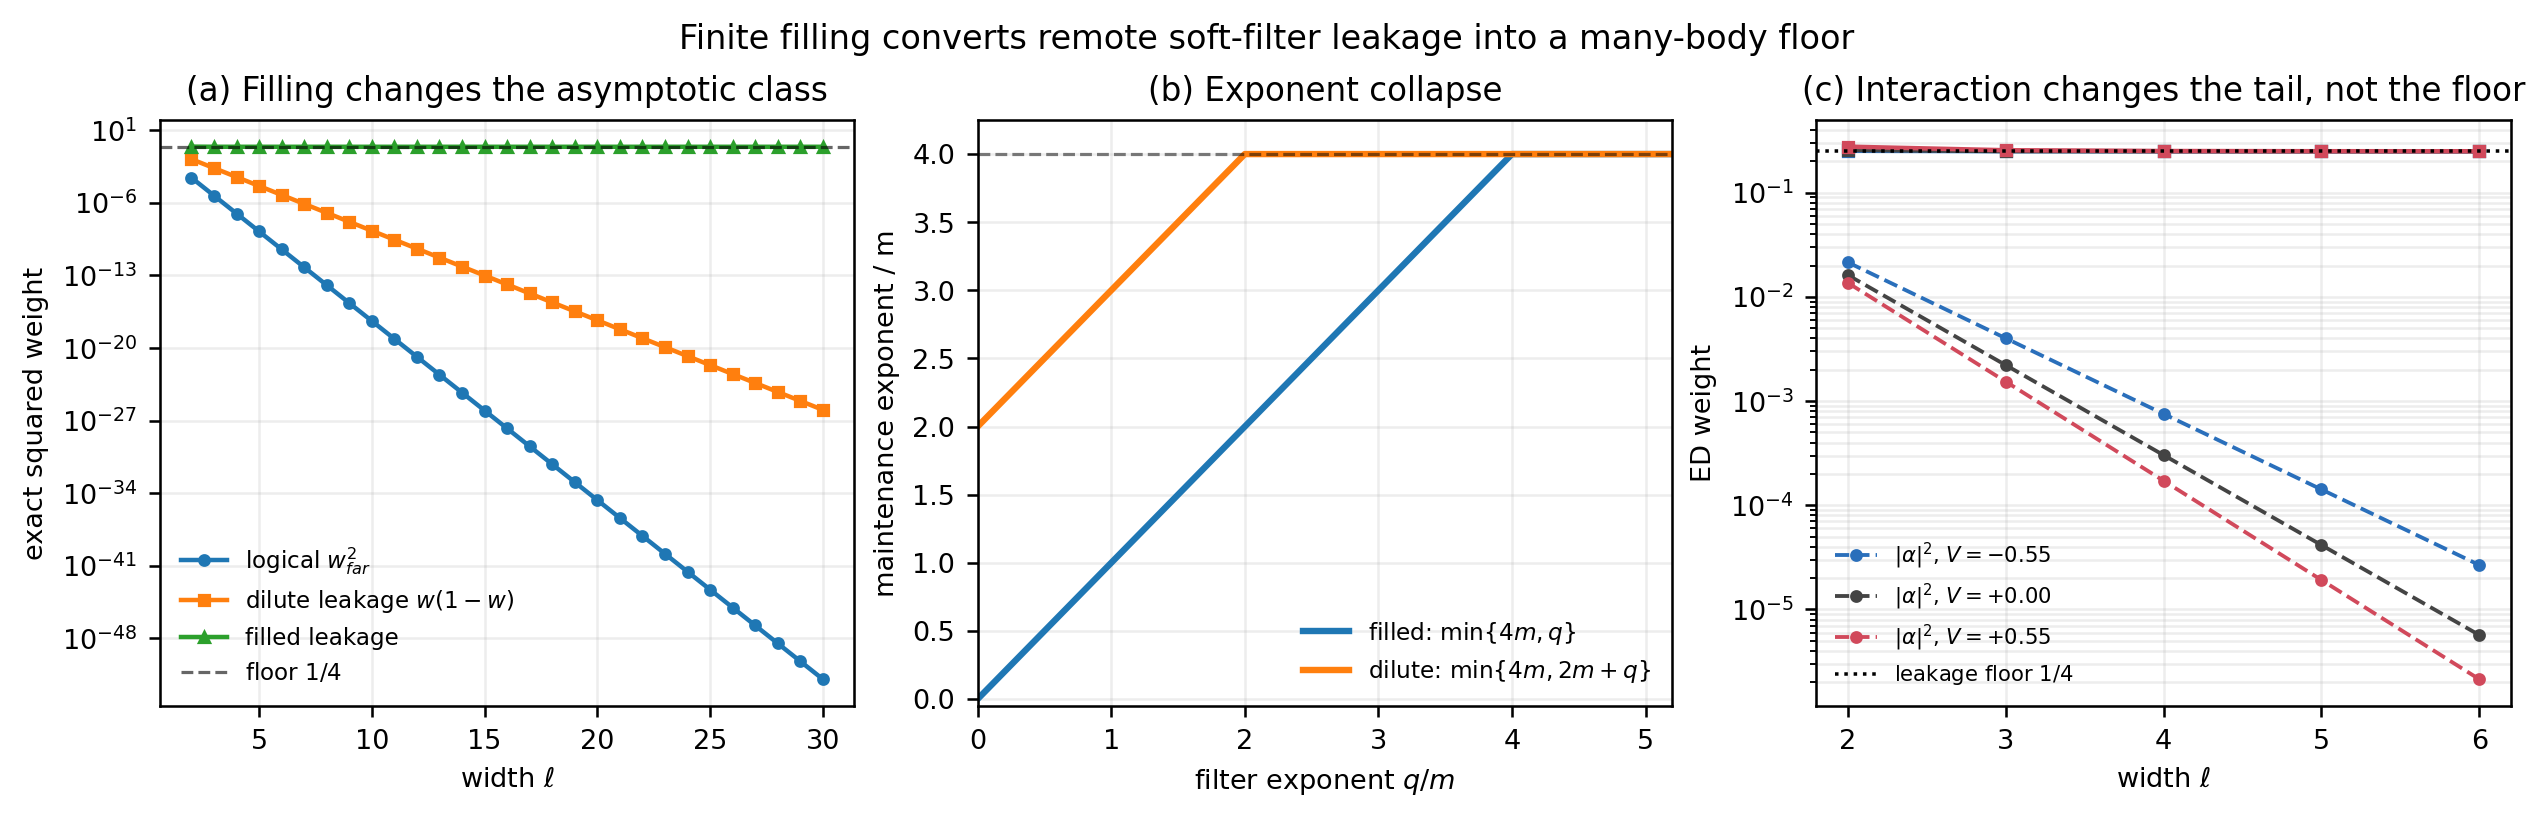
\includegraphics[width=\textwidth]{many_body_filling_phase_diagram.png}
\caption{Left: exact remote logical and leakage weights in the dilute and half-filled SSH codes.  Center: filter-exponent phase diagrams; finite filling changes the leakage branch from $2m+q$ to $q$.  Right: exact diagonalization of the interacting spinless SSH rail.  Interactions change the edge localization slope while the leakage retains its $1/4$ floor.}
\label{fig:phase}
\end{figure}

\section{Scope, falsification, and implications}

The exact free result is falsified by any violation of \cref{eq:wleak} under the stated filling and boundary transfer.  The interacting theorem is falsified if its occupation product stays bounded below and its logical matrix element vanishes, yet the projected leakage does not retain a floor.  The spectral-window result is a direct moment inequality and can fail only if the commutator bound or the spectral-band hypothesis is removed.

Several limitations are explicit:
\begin{itemize}
\item The Davies generator is constructed after taking the weak-coupling limit at each fixed width; no uniform pre-Davies limit is proved.
\item The exact exponent equality $\min\{4m,q\}$ is proved for the free filled SSH family.  The interacting theorem proves a stable leakage floor and a Davies lower bound, but not a universal interacting logical exponent.
\item The bath lower envelope on a compact nonlogical window is an assumption.  The local spectral-window lemma makes that window width independent but does not derive the reservoir spectrum.
\item The fixed-latency equality uses a fresh-target-cell resource ledger.  It is not an autonomous work-only controller theorem.
\item The result concerns a boundary transfer.  A controller engineered to annihilate the filled background before transferring the edge charge implements a different system operator and may evade the floor at an additional resource cost.
\end{itemize}

The practical conclusion is sharper than in the dilute model.  Perfect filtering was already the boundary between finite and singular rapid exact maintenance.  At finite filling, imperfect filtering also determines whether widening the membrane helps at all.  A constant tail does not merely reduce the exponent: it removes it.

\appendix

\section{Fermionic tensor factors}

The two rails are combined with the graded tensor product.  The operator $S_x=a_{1,x}^\dagger a_{0,x}$ is even and preserves total number.  Matrix elements between fixed-total-number code states may acquire a convention-dependent uniform sign from ordering the rails, but every weight used in the paper is a modulus square.  Moreover,
\[
 S_x^\dagger S_x
 =a_{0,x}^\dagger a_{1,x}a_{1,x}^\dagger a_{0,x}
 =a_{0,x}^\dagger(1-n_{1,x})a_{0,x}
 =n_{0,x}(1-n_{1,x}),
\]
because the even operator $n_{1,x}$ commutes with the rail-zero fields.  Thus no hidden fermionic sign enters the occupation identities.

\section{Free spectral decomposition of the leakage}

Expand the boundary field as
\[
 a_x=\psi_x f_0+\sum_k u_{k,-}(x)f_{k,-}+\sum_k u_{k,+}(x)f_{k,+}.
\]
In $|e_\ell\rangle$, the zero and negative modes are occupied; in $|g_\ell\rangle$, only the negative modes are occupied.  Therefore $S_x|0_L\rangle$ contains exactly four types of terms.  The zero-to-zero term is logical.  Orthogonality of the Slater determinants makes all other terms mutually orthogonal after summing over band labels.  Lemma~\ref{lem:chiral} gives
\[
 \sum_k|u_{k,-}(x)|^2
 =\sum_k|u_{k,+}(x)|^2
 =\frac{1-w_x}{2},
\]
which yields the three leakage rows displayed after \cref{thm:filledidentity}.  This derivation also shows that degeneracies of particle--hole Bohr frequencies cannot create a multiplicity factor: coherent recombination within a degenerate frequency block preserves the same total squared norm.

\section{Resource ledger}

For completeness, the fixed-period achievability statement uses a cell whose Hamiltonian is isomorphic to the logical-plus-bulk system and whose initial state is a fresh copy of the target.  A number-conserving graded SWAP exchanges system and cell.  If the discarded system state after free evolution is $\sigma$, the minimum reversible work of re-preparing the cell is
\[
 F(\rho)-F(\sigma)
 =k_{\mathrm B}T\bigl[D(\rho\Vert\gamma)-D(\sigma\Vert\gamma)\bigr].
\]
This ledger proves equality inside a permissive collision-model class.  It consumes target-state resources and must not be conflated with ordinary work-only autonomous stabilization.

\clearpage
\small
\begin{thebibliography}{99}
\setlength{\itemsep}{0.15em}

\bibitem{Davies}
E.~B. Davies,
``Markovian master equations,''
\emph{Commun. Math. Phys.} \textbf{39}, 91--110 (1974),
doi:10.1007/BF01608389.

\bibitem{Spohn}
H. Spohn,
``Entropy production for quantum dynamical semigroups,''
\emph{J. Math. Phys.} \textbf{19}, 1227--1230 (1978),
doi:10.1063/1.523789.

\bibitem{GraceGuha}
M.~R. Grace and S. Guha,
``Perturbation theory for quantum information,''
arXiv:2106.05533.

\bibitem{SSH}
W.~P. Su, J.~R. Schrieffer, and A.~J. Heeger,
``Solitons in polyacetylene,''
\emph{Phys. Rev. Lett.} \textbf{42}, 1698--1701 (1979),
doi:10.1103/PhysRevLett.42.1698.

\bibitem{MonkmanSirker}
K. Monkman and J. Sirker,
``Operational entanglement of symmetry-protected topological edge states,''
\emph{Phys. Rev. Research} \textbf{2}, 043191 (2020),
arXiv:2005.13026.

\bibitem{ErikssonLeakage}
L. Eriksson,
``Support Leakage Makes Rapid Quantum Maintenance Singular: Soft Spectral Filters and Exponent Transmutation in Dual-Rail SSH Codes'' (2026),
\url{https://github.com/lluiseriksson/support-leakage-rapid-maintenance}.

\bibitem{JinRuggieroGiamarchi}
T. Jin, P. Ruggiero, and T. Giamarchi,
``Bosonization of the interacting Su--Schrieffer--Heeger model,''
arXiv:2301.00472.

\bibitem{HastingsWen}
M.~B. Hastings and X.-G. Wen,
``Quasi-adiabatic continuation of quantum states: The stability of topological ground-state degeneracy and emergent gauge invariance,''
\emph{Phys. Rev. B} \textbf{72}, 045141 (2005),
arXiv:cond-mat/0503554.

\bibitem{BachmannEtAl}
S. Bachmann, S. Michalakis, B. Nachtergaele, and R. Sims,
``Automorphic equivalence within gapped phases of quantum lattice systems,''
\emph{Commun. Math. Phys.} \textbf{309}, 835--871 (2012),
arXiv:1102.0842.

\bibitem{MoonNachtergaele}
A. Moon and B. Nachtergaele,
``Stability of gapped ground state phases of spins and fermions in one dimension,''
\emph{J. Math. Phys.} \textbf{59}, 091415 (2018),
arXiv:1804.04750.

\bibitem{ShtankoEtAl}
O. Shtanko, Y.-J. Liu, S. Lieu, A.~V. Gorshkov, and V.~V. Albert,
``Bounds on autonomous quantum error correction,''
arXiv:2308.16233.

\bibitem{VacantiEtAl}
G. Vacanti, C. Elouard, and A. Auff\`eves,
``The work cost of keeping states with coherences,''
arXiv:1503.01974.

\end{thebibliography}

\end{document}
